149. \begin{figure}[ht!]
\center{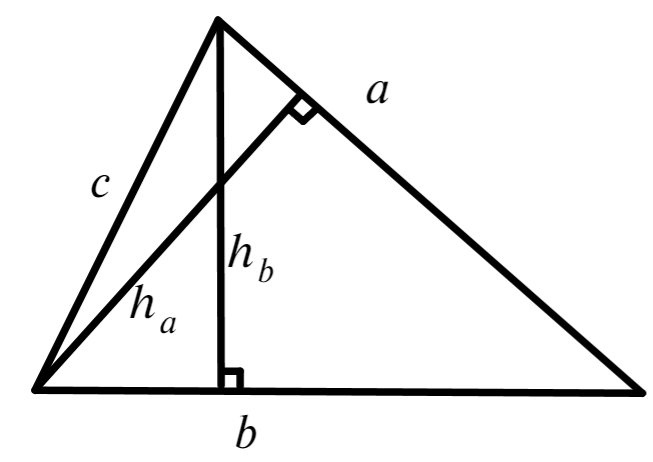
\includegraphics[scale=0.35]{g7-149.png}}
\end{figure}\\
Пусть к сторонам $a$ и $b$ проведены высоты $h_a$ и $h_b.$ Учитывая условие и то, что перпендикуляр не превосходит наклонную, получим цепочку неравенств $a\leqslant h_a\leqslant b \leqslant h_b \leqslant a.$ Значит, все неравенства должны обращаться в равенства и треугольник является прямоугольным (так как высоты совпадают со сторонами) и равнобедренным (так как равны две стороны). Тогда его углы равны $45^\circ,\ 45^\circ$ и $90^\circ.$\\
